\section{Naive implementation}
Naive implementation was made as a proof of concept. Process of implementation is pretty straightforward. Structure contains two tries for odd and even palindromes, current maximum palindromic suffix and sequence before that suffix. To add a new symbol to the tree we generate palindromic suffix candidates for input symbol. If symbol before that suffix and input symbol are same, that means that we found a new palindrome, update max palindromic suffix and add new node to the proper trie. If none of candidates is suitable, symbol simple adds to odd trie after the root. 

To check that it works, we can calculate number of rich palindromes of length $n$ and compare it with actual sequence from OEIS \cite{oeisA216264}. A sequence of length $n$ is called rich if it contains, as subsequences, exactly $n$ distinct palindromes. Also we will use this method of checking further during project.

Code for that implementation can be found in GitHub repository\cite{khazhix3}.
\section{Two sided tree}
As the original tree \cite{RUBINCHIK2018249} holds only maximum palindrome suffix, we can only append a new symbol. But what if we want to add a new symbol at the beginning? To allow that we can add maximum palindrome prefix support. So we might need to keep track of max prefixes, but as palindrome is symmetric, maximum palindrome suffix of palindrome is maximum palindrome prefix as well. Thus we can simply keep information about maximum palindrome prefix of processed string (as we keep information about maximum suffix). So no major memory usage is added, only one more entry.

This extension allows us merge two eertrees more efficient than simple naive approach (adding symbol by symbol from string of eertree$_2$ to eerteee$_1$). Let's consider example: $"abbabba" + "bbbab"$.
Palindromes of concatenated string includes all processed palindromes of both strings and new ones. It's pretty obvious that new palindromes can be found somewhere around joint of two strings. 

There are three cases: \begin{enumerate*}
  \item center of new palindromes is joint
  \item center of new palindromes is max suffix (and/or its max suffixes) of first string
  \item center of new palindromes is max prefix (and/or its max prefixes) of second string.
\end{enumerate*}
For current example blue represents max palindrome prefix, red represents max palindrome suffix and black represents symbols that we are checking:
$"\mathunderline{red}{abb\mathunderline{red}{abb\mathunderline{red}{a}}}" + "\mathunderline{blue}{\mathunderline{blue}{\mathunderline{blue}{b}b}b}ab"$
\begin{enumerate}
\item $"abbabb\underline{a}" + "\underline{b}bbab"$, $"ab"$ is not a palindrome, stop here.
\item $\underline{\ \ }"\mathunderline{red}{abb\mathunderline{red}{abb\mathunderline{red}{a}}}" + "\underline{b}bbab"$, nothing to compare, moving to next max suffix \\
$"ab\underline{b}\mathunderline{red}{abb\mathunderline{red}{a}}" + "\underline{b}bbab"$, $"babbab"$ is potential new palindrome, expanding more\\
$"a\underline{bb}\mathunderline{red}{abb\mathunderline{red}{a}}" + "\underline{bb}bab"$, $"bbabbabb"$ is potential new palindrome, expanding more\\
$"\underline{abb}\mathunderline{red}{abb\mathunderline{red}{a}}" + "\underline{bbb}ab"$, $"abbabbabbb"$ is not a palindrome, moving to next max suffix.\\
$"abbab\underline{b}\mathunderline{red}{a}" + "\underline{b}bbab"$, $"bab"$ is potential new palindrome, expanding more\\
$"abba\underline{bb}\mathunderline{red}{a}" + "\underline{bb}bab"$, $"bbabb"$ is potential new palindrome, expanding more\\
$"abb\underline{abb}\mathunderline{red}{a}" + "\underline{bbb}ab"$, $"abbabbb"$ is not a palindrome, stop here.
\item 
$"abbabb\underline{a}" + "\mathunderline{blue}{\mathunderline{blue}{\mathunderline{blue}{b}b}b}\underline{a}b"$, $"abbba"$ is potential new palindrome, expanding more\\
$"abbab\underline{ba}" + "\mathunderline{blue}{\mathunderline{blue}{\mathunderline{blue}{b}b}b}\underline{ab}"$, $"babbbab"$ is potential new palindrome, expanding more\\
$"abba\underline{bba}" + "\mathunderline{blue}{\mathunderline{blue}{\mathunderline{blue}{b}b}b}\underline{ab\ \ }"$, nothing to compare, moving to next max prefix \\
$"abbabb\underline{a}" + "\mathunderline{blue}{\mathunderline{blue}{b}b}\underline{b}ab"$, $"abbb"$ is not a palindrome, moving to next max prefix\\
$"abbabb\underline{a}" + "\mathunderline{blue}{b}\underline{b}bab"$, $"abb"$ is not a palindrome, stop here\\
\end{enumerate}
All found palindromes are added to the a tree. Max palindrome suffix of merged tree is max palindrome suffix of second string. If one of new found palindromes includes whole second string, it becomes max palindrome suffix. And visa-versa max palindrome prefix of merged tree is max palindrome prefix of first string. If one of new found palindromes includes whole first string, it becomes max palindrome prefix. Thus max suffix can be same sequence as max prefix. 

Another paper from Rubichik \cite{rubinchik2016number} showed that random word of length $n$ contains, on expectation, $\Theta(\sqrt{n})$ distinct palindromic factors. So if length of first string is $n$ and length of second is $m$, on expectation, their concatenation gives us $\Theta(\sqrt{n + m})$ palindromes. From that we exclude palindromes that already processed separately. Since max palindrome suffix and prefix can be new palindromes from concatenation we can update them both at $O(\sqrt{n + m})$.   
\section{Infinite tree}
In the original paper author proposed a persistent version of tree, but it based around global mutable structure. We could also achieve persistency using naive implementation, but in that case we need to copy whole structure since there are cyclic dependencies, that is inefficient. To achieve persistency we need to approach a little bit different. 

For some alphabet $\sigma$ we can simply generate palindromes of length $n$. The number of palindromes of length $n$ will be $g(n, \sigma)$ where 
$$g(n, \sigma) = \begin{cases}
\ \sigma^{\frac{n+1}{2}}  & n \ is \ odd\\
\ \sigma^{\frac{n}{2}}   & n \ is \ even
\end{cases}$$
 That infinite tree will represent all possible palindromes and their dependencies. That tree, in fact, is variation of joint eertree proposed in original paper. So the number nodes of infinite tree for fixed alphabet will be $\sum_{n=1}^{\infty} g(n, \sigma)$. Here where haskell's lazy evaluation will come in handy. We need to calculate only certain subtree from that tree and it will use $O(n)$ memory. 
 
 Unary infinite tree was implemented\cite{fizruk}.
\begin{figure}[H]
  \centering
     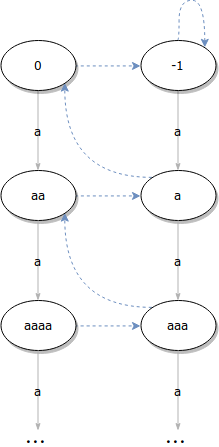
\includegraphics[width=0.4\linewidth]{unary.png}
 \caption{Infinite tree over unary alphabet}
\end{figure}
\begin{figure}[H]
  \centering
     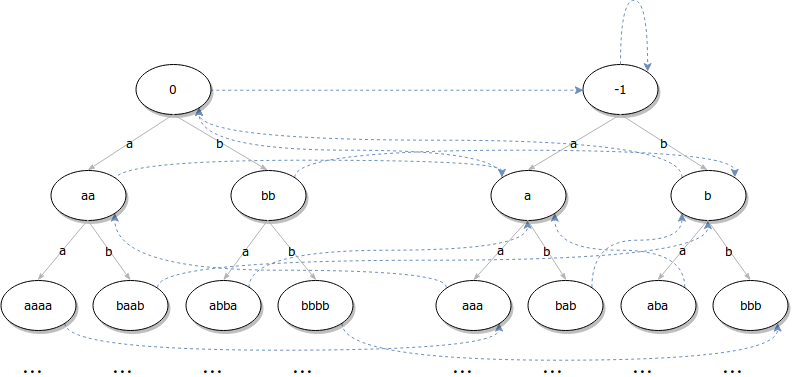
\includegraphics[width=\linewidth]{binary.png}
 \caption{Infinite tree over binary alphabet}
\end{figure}
